\documentclass[12pt]{article}
\usepackage[utf8]{inputenc}
\usepackage[english, russian]{babel}
\usepackage{graphicx}
\usepackage{setspace,amsmath}
\begin{document}
	\subsection*{Представление работы программы}
	
	Все шаги описаны в книге, и там же указано, как нужно представлять результаты вычислений в виде графиков. Поэтому здесь представлены только они, чтобы показать работоспособность программы на наборе данных, идентичном тому, что описан в учебнике, за исключением шума, разумеется.
	
		\begin{figure}[h]
			\centering
			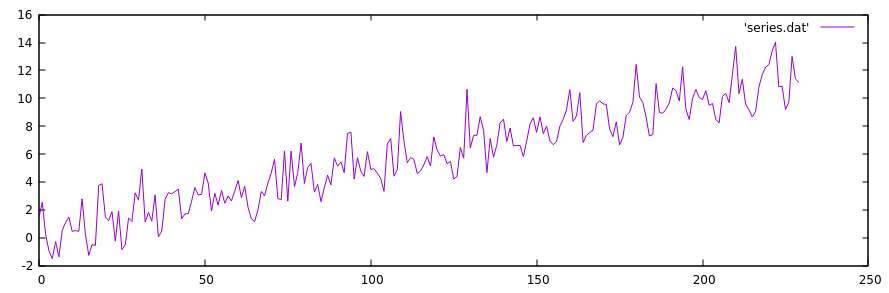
\includegraphics[width=14cm]{justseries.png} 
			\caption{Модельный временной ряд} 
			\label{fig.0} 
		\end{figure}
		
		\begin{figure}[h]
			\centering
			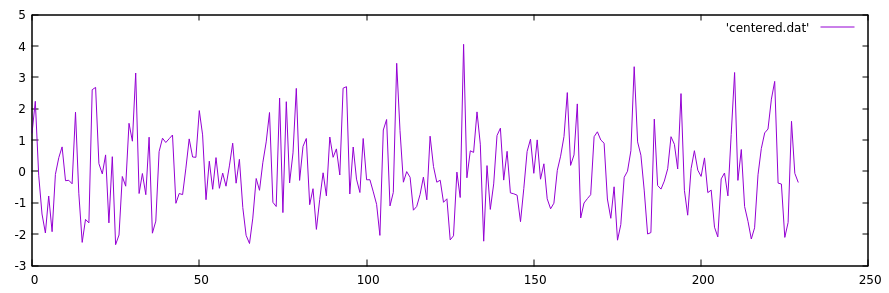
\includegraphics[width=14cm]{centered.png} 
			\caption{Центрированный временной ряд} 
			\label{fig.0} 
		\end{figure}			

		\begin{figure}[h]
			\centering
			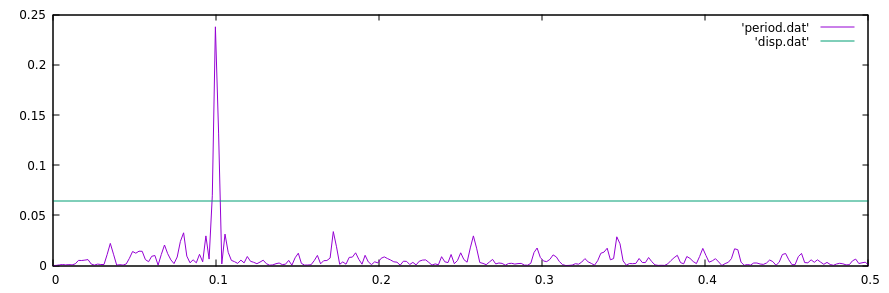
\includegraphics[width=13cm]{period.png} 
			\caption{Периодограмма и уровень q=0.01} 
			\label{fig.0} 
		\end{figure}
	
		\begin{figure}[h]
			\centering
			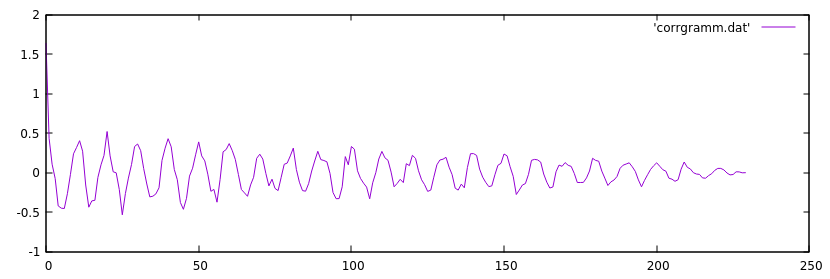
\includegraphics[width=13cm]{corrgramm.png} 
			\caption{Коррелограмма} 
			\label{fig.0} 
		\end{figure}

		\begin{figure}[h]
			\centering
			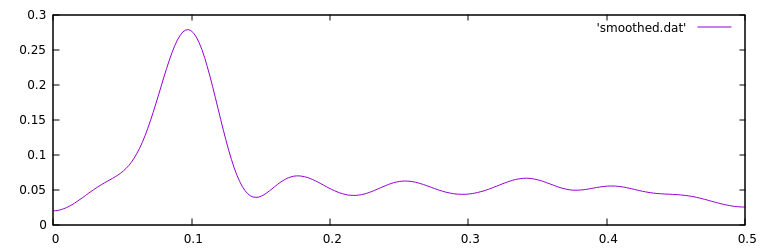
\includegraphics[width=13cm]{smoothed.png} 
			\caption{Сглаженная периодограмма} 
			\label{fig.0} 
		\end{figure}



\

\

\

\

\

\

\

\

\

\

\

\

\newpage

	\subsection*{Задание}
	Задание: продемонстрировать вероятность того, что наибольший отсчет периодограммы дискретного белого шума превысит заданный уровень $X_1$ (определяемый уравнением (24) из учебника). 
	
	Программа Спектрально-корреляционного анализа временных рядов была вызвана в роли процедуры 100-200 раз с исходным рядом, являющимся смоделированным белым шумом. Для визуализации вероятности появления пика у белого шума на периодограмме с уровнем значимости, соответствующим $q=0.01$, программа построила периодограмму для шума, нашла ее максимальный отсчет и разность с уровнем значимости.
	
	 Предполагается, что при наличии какого-нибудь сигнала, пик, соответствующий его частоте на периодограмме, внесет существенный вклад в повышение уровня значимости, так как будет участвовать в расчете дисперсии. Однако, в данном случае на вход подается чистый шум, что может несколько снизить уровень, и в итоге может оказаться, что слишком много пиков у шума превышают этот уровень. Тем не менее, программа выдает удовлетворительные результаты визуализации и в этом случае. 
	 
	 На рис.6 и 7 представлены графики, где каждая пара точек, соответствующая одной абсциссе, отображает наибольший отсчет периодограммы для конкретного одного запуска программы с белым шумом на входе (номер этого запуска и является координатой-абсциссой) и уровень значимости ($q=0.01$ и $q=0.05$ для рис.6 и 7 соответственно). В первом случае программа запускалась 200 раз. Было зафиксировано два случая, где наибольший отсчет периодограммы превышает уровень. 2 случая из 200 как раз и соответствует вероятности $q=0.01$ принять пик, созданный шумом, за сигнал. 
	 
	 Для второго случая с $q=0.05$ ситуация такая же. Было зафиксировано 5 случаев, где наибольший отсчет периодограммы превышает уровень значимости. 5 случаев из 100, в свою очередь, соответствует вероятности $q=0.05$ принять пик, созданный шумом, за сигнал.
	 
	 Таким образом, можно весьма наглядно продемонстрировать данную вероятность принятия шумового пика за пик, принадлежащий сигналу, с заданным уровнем значимости, если просто запустить программу, генерирующую белый шум и вычисляющую для каждого ряда из шумов свою периодограмму и свой уровень значимости, сравнивая их друг с другом. При большом количестве запусков программы, в пределе стремящемся к бесконечности, количество случаев превышения отсчетов периодограммы шума над уровнем значимости, деленное на общее количество запусков, стремится к установленной заранее вероятности $q$.

		\begin{figure}[h]
			\centering
			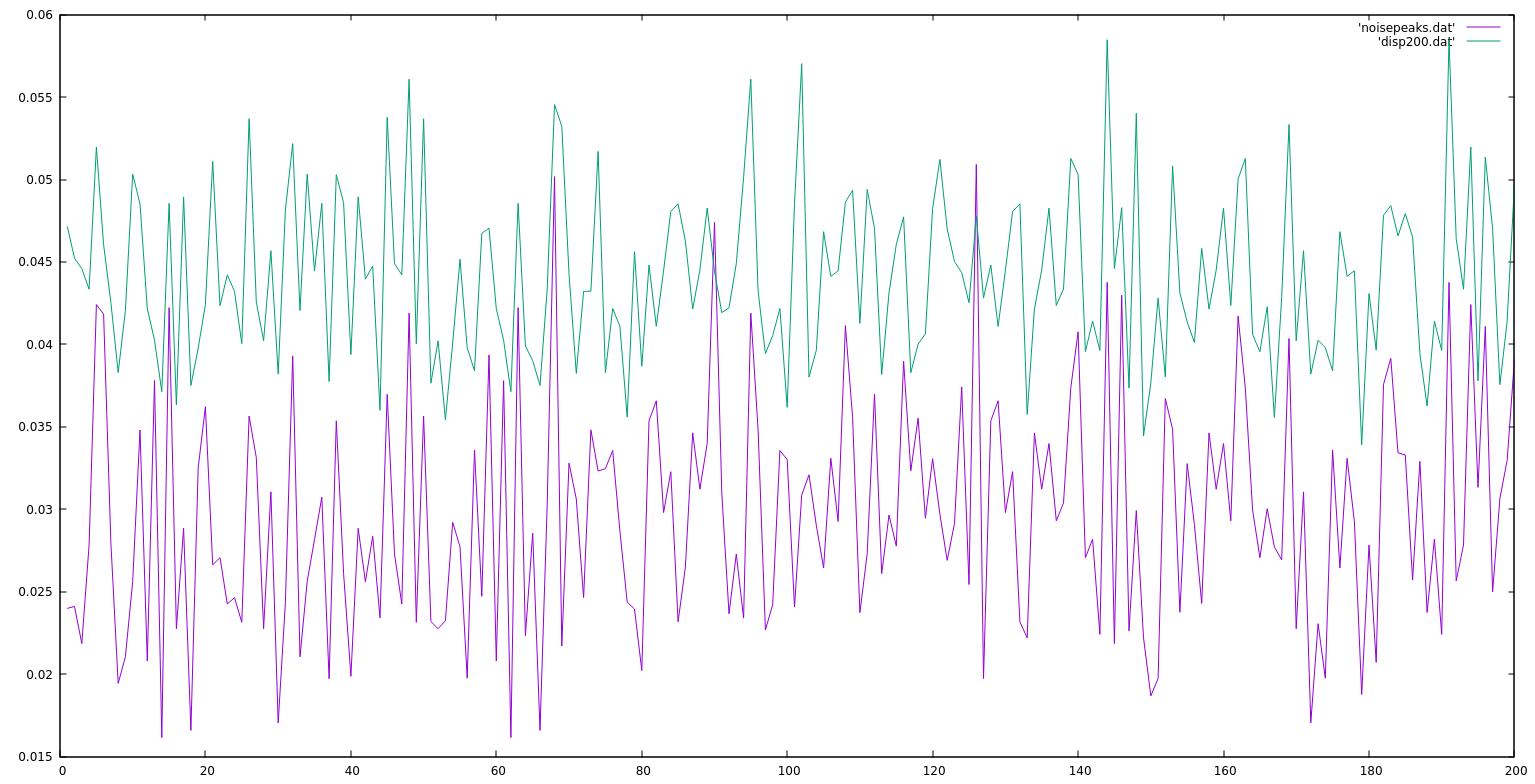
\includegraphics[width=14cm]{peaksdisp.png} 
			\caption{Наибольшие отсчеты периодограммы чистого белого шума и уровень q=0.01 для 200 вариаций шума} 
			\label{fig.0} 
		\end{figure}		

		\begin{figure}[h]
			\centering
			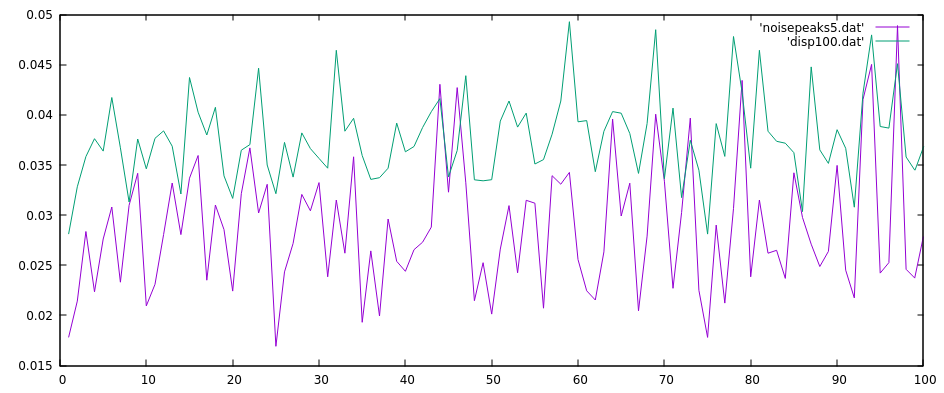
\includegraphics[width=14cm]{peaksdisp5.png} 
			\caption{Наибольшие отсчеты периодограммы чистого белого шума и уровень q=0.05 для 100 вариаций шума} 
			\label{fig.0} 
		\end{figure}		
				
		
		

\end{document}